\documentclass[a4paper]{IEEEtran}
\usepackage{hyperref}
\usepackage{url}
\usepackage{graphicx}

\begin{document}
\author{Catalin David}
\title{Channel Modelling Using Bellhop in Underwater Acoustic Sensor Networks}

\maketitle
\begin{abstract}
To develop a seabed of underwater acoustic sensor network is very
challenging. Moreover, due to the costs and effort required to deploy
such a network, it is imperative to understand how the acoustic
channel behaves in an underwater environment and be able to simulate
the exact behavior of the network before deployment.
Therefore, it is of great importance to know the
specifics of the environment and to use a good modelling tool.
In this paper we describe a step by step procedure on how to experiment and
evaluate channel conditions in an underwater environment modelled by
the Bellhop tool, part of the Acoustic Toolkit.
\end{abstract}

\section{Introduction}
Studying and modelling how underwater sensor networks behave is a new and
difficult task, but the rewards are incredible: exploration of the ocean which
covers about 70\% of the earth surface -- this will ease the search of new
energy sources, it will allow environmental and industrial monitoring (of
animals and equipment), early disaster warning (for earthquakes, tsunamis) and,
of course, for other military purposes.

While the design of such a system might seem related to the one of terrestrial
networks, it is very different. Unlike the terrestrial counterpart, for
underwater networks only acoustic communications are considered to be viable (at
the physical layer) and this creates issues, since in the terrestrial setting
you have radio frequency (RF) communications. In an underwater environment, RF
has been tested and the results were not very good, the transmission suffering
from severe atenuation, the only succesful deployment being at very low
frequencies and with a large antenna and a very high transmission power. Still,
this is not what one would have in mind when thinking about an underwater sensor
network: an underwater sensor network consists of many interlinked sensors that
are deployed once and with which there is no physical interaction for a long
period of time. This generates many requirements, but the most important for the
networking part are energy efficiency and a reliable transmission, leading to
the study of acoustic channels.

From a networking point of view, the acoustic communication is very different
from the RF communication, mainly due to the low bandwidth, propagation delay
and the quality of the link. One other important thing to note is that
underwater networks are, in general, very prone to noise due to the environment
-- waves, shipping activity, a modification in the temperature or salinity of
the water etc. We consider now a network with multiple nodes in which there
might be multiple paths between each destination and receiver. If terrestrial
protocols were to be used in such a volatile environment, when a link would be
down, there would be an increased amount of traffic in the network for rerouting
the transmission of data, leading to a high energy usage, ignoring one of the
main requirements.

Since the development and deployment costs for such a network, alognside with
the limited remote access to the deployed network,  one of the challenges
involved is to develop a valid simulation model that is able to provide results
that are according to real life. Once that is done, one can experiment with
different theoretical implementations and find out more about the underwater
communication constraints and limits.

\section{Background}
\subsection{Motivation}
In order to deploy an underwater network, one needs both financial and time
resources, as it is a very expensive and difficult task. Therefore, prior to the
deployment of such a network, all efforts need to be made in order to find new
ways to deal with the challenges of such an environment. This motivates
researchers to find models that try to simulate as well as possible the
conditions of the seabed (where the network will most likely be deployed).

Some of the challenges found in the underwater environment are long latency and
limited bandwidth, a high degree of noise, high bit error rates and transmission
loss, reliability, energy and cost constraints, as well as volatile link
quality. A few of these are briely explained below.

\textit{Long Latency and Limited Bandwidth}: The acoustic channel in the
underwater environment is characterized by long latency and limited bandwidth.
The speed of propagation of acoustic waves ($1.5 x 10^3 m/s$) is five orders of
magnitude lower than the one specified for an RF environment. For this, we need
to consider the propagation range, which can vary between few meters and many
kilometers. In any case, the bit rate for such a channel is very low.

\textit{Noise, High Bit Error Rates and Transmission Loss}: The underwater
environment is subject to a lot of noise coming from different sources, such as
turbulences, wind, shipping activity and thermal effects, as well as seismic
activity, fishes swimming. The model has to be very elastic with regards to all
these factors which, in real life, can actually produce communication failure
over certain links. Even without noise, a model has to take into consideration
the attenuation (transmission loss) of the signal, which increases with both
distance and frequency, as well as geometric spreading.

\textit{Energy and Cost Constraints}: Deploying a network of underwater nodes is
much more complicated than deploying the same network in the terrestrial
environment. The biggest constraints are that in the underwater environment, the
node casing has to resist a great pressure and that the nodes should be
independent of human activity (it is costly to take out and put back the nodes
every day). Moreover, light sources are not available at such depths, resulting
in a system that has to be very energy efficient. Coupling that with such a bad
channel quality, in which the communication protocols might fail, which results
in retransmission, we get a very high amount of used energy.

As previously noted, all these factors, all these constraints motivate people to
try even more to find new ways to communicate underwater, to better understand
the transmission specifics for this environment, to develop new technologies and
models before committing to actually deploying such a network.

\subsection{Previous Work}
As stated before, the need for understanding the characteristics of
communication in an underwater channel is one of the basic prerequisites in
order to create better underwater sensor networks. Still, the experiment
conducted does not focus on a general approach towards modelling the entire
environment, but we are focusing on a specific region (near the bottom of the
sea). The experiment in this article is based on real data (fed into the Bellhop
modelling tool \cite{bellhop}) and tries to be as close to reality as possible,
by using multipath for signal analysis -- which is relevant since we are talking
about the bottom of the sea where reflections from the seabed are possible.

The work of M. Stojanovic \cite{stojanovic} is very relevant to this field, as
it documents the theoretical background behind underwater channel analysis. This
article synthesises the required mathematical background, as well as channel
analysis knowledge. Since this article is of high relevance in the field and is
acknowledged to be one of the best, this allows us to use the theory and
calculations documented to reach the desired results.

The purpose of the experiment is to reproduce the results provided by
\cite{book} so that they can be used later on in the related paper: \cite{nds}.
We base our experiment on the data from the article. Relevant work is also
documented in \cite{hayward}, where the authors also try to determine the
channel characteristics (bandwidth and channel capacity), but unlike the work
documented here, their research is based on communication links in the upper
half of the water column.

An alternative to using a ray-tracing algorithm such as Bellhop is to use the
NS-2 simulator and extend it to adjust to the underwater environment. Such a
model has been implemented, by extending the NS-2 simulator (see \cite{ns2}) and
has provided great results, with a very small amount of used computation time.
Still, due to the nature of the simulator, the data is not similar to the one
obtained from a ray-tracing algorithm, since NS-2 uses a single path from source
to destination (similar to a water rippling effect), while a ray-tracing
algorithm provides multipath and a more in-depth analysis of the data (one can
find out the exact path that the ray went through to reach the destination, the
phase shift of the signal and how it contributes to the final impulse response).

\section{Methodology}
A number of steps need to be taken in order to achieve the results. First of
all, data that describes the environment needs to be collected. This data is
then transformed to a computer-understandable format for the modelling tool
(Bellhop program) to understand it. Then the modelling tool interprets this data
and runs, generating the output. This output will then have to be postprocessed
in order to compute the channel characteristics. Since we are committed to using
the Bellhop program for ray-tracing, part of the Ocean Acoustic Library
\cite{oal}, we will describe the process in a detailed way for this modelling
tool. Still, if one wishes, another modelling tool can be used, but this will
have impact with regards to the preprocessing and postprocessing of the data
(but the general workflow will be the same.

\subsection{Preprocessing the Environment}

The Bellhop program uses as input environment files (usually with extension
ENV). An environment file serves as a description of how the environment behaves
at certain parameters, as well as to instruct the Bellhop program what output
data is required, in what format the data will be output, all according to a
certain template. The environmental file comprises of a few ``sections'' that
describe characteristics of the environment, such as sound speed profile and
bathymetry. These sections of environmental file are presented below in theory,
as well as as how they look in our model, in section \ref{sec:case}.

\subsubsection{Frequency}
One constraint (or feature) of the Bellhop tool is that it can only use one
frequency at which it operates. Therefore, in order to perform a multi-frequency
analysis, one must define multiple input files, one for each frequency. The
start, end and step frequency are to be determined by the user, depending on the
use and wished granularity of the output. The main impact of this paramater is
over the transmission loss (or attenuation) of the signal, as this higly
dependant on the frequency in an underwater environment.

\subsubsection{Sound Speed Profile}
Since we are using acoustic waves and an inhomogeneous propagation environment,
this system has to obey Snell's law of propagation: $$ \frac{\cos{\theta}}{c} =
constant $$

This means that the acoustic rays will not travel in a straight line, but they
will bend towards the areas of lower speed. This data can be generated, but it
is better if this data actually comes from real measurements near the
area of interest. In general, the speed of sound is not revealed by
measurements, but it is described in term of other measurements by the
following equation: 
\begin{eqnarray*}
 c = 1449.2 + 4.6 T - 0.055 T^2 + 0.00029 T^2 +\\
(1.34 - 0.01 T)(s - 35) + 0.06z
\end{eqnarray*}
where $T$ stands for temperature (in Celsius degrees), $s$ is salinity
in Practical Salinity Units (PSU) and $z$ is the depth (meters) -- in
fact, this formula is not complete; the complete version of this
formula can be found in \cite{ssp}, but this represents a good
approximation. 
Therefore, in order to find the speed of sound at different depths, we
only need the salinity and temperature measurements for a certain
area. These values can usually be obtained via the Bedford Institute
of Oceanography (BIO) \cite{bio} or via the National Oceanic and
Athmospheric Administration (NOAA) \cite{noaa}. Still, these values
are not stable, as the temperature might vary during the day, month, season or
year, so the SSP must be generated either from averaged values for these
parameters or the SSP can be specific to a certain time, case in which
one would only take into consideration a specific scenario.

\subsubsection{Bottom Description}
In our modelled scenario, we have an interest in sound propagation
near the bottom of the sea. Since we are using the Bellhop program
which performs ray-tracing, thus taking into consideration multiple
paths between the source and the destination, we need to provide the
program a description of the seabed. The description must be given in
terms of three components: how the sound propagates through the
seabed, how rough is the terrain and what is the bathymetry of the
region of interest.

The first option refers to the way acoustic rays interact with the
seabed. The seabed can be considered to be a vacuum-like surface
(sound does not propagate through), a perfectly reflective surface or
it can have a more complicated description.

The roughness of the terrain is given as a root-mean-squared (RMS)
value in meters of the inter-facial features of the sea bottom. The
last parameter is the actual bathymetry of the seabed -- this has to
be provided in an additional file (BTY), one per each ENV file
corresponding to a single direction.

\subsubsection{Sources, Receivers, Ranges}
In the ENV file, multiple sources, multiple receivers and multiple
ranges can be specified. Ray-tracing is performed between only a
sender and a receiver, each of which is characterized by a depth and
the entire system is characterized by a distance between the
nodes. Using Bellhop, we can specify multiple depths for the sources,
multiple depths for the receivers and multiple distances between the
sender and receiver, meaning that ray-tracing can be computed
for multiple $\langle source,receiver,range \rangle$ tuples. Since
ray-tracing is performed for each of these tuples, that means there
are $$\#sources \times \#receivers \times \#ranges$$ possibilities for which the
program must be run, thus yielding a direct proportionality between each of
the number of sources, receivers and ranges and the final runtime of
the program.

\subsubsection{Run Type}
The Bellhop program is designed with many options with regards to the
type of computations that it can perform and also with regard to the
type and format of the output. There are three main types of output
that Bellhop can provide: ray, amplitude-delay and acoustic field.

Ray files contain the exact path of the rays that travel between the
source and the destination. The amplitude-delay files contain
information about each ray that travels between source and destination
in terms of strength, phase shift and delay at the destination. The
last type, acoustic field is used to describe the ocean as an actual
acoustic field in which the most important information is the relative
signal strength within the desired area. For this experiment, we are
interested in the amplitude-delay output of Bellhop.

\subsubsection{Beam Width}
In order to limit and reduce the number of rays for which the path
must be calculated, we can impose a restriction at the source on how
wide the beam should be. This can be done by providing a minimum and
maximum angle between which the rays can start propagating from the
source. The values for these angles can be both negative, case in
which this is an angle towards the surface of the water, or
positive, case in which this is an angle towards the bottom. Besides
these angles, we can also provide the number of beams that will start
from the source within this range or we can let Bellhop decide what
the best value is.

\subsubsection{Bounding Box}
Ray-tracing is a very time and processor-intensive operation,
therefore, a bounding box has been introduced to further reduce the
amount of rays that can be followed. Still, if a too small bounding
box is used, this can interfere with the ray-tracing algorithm (as
some of the rays exit the bounding box), so the recommended bounding
box should extend slightly behind the bottom depth and behind the
maximum range.
\subsection{Arrival Analysis and Data Interpretation}
We skip ahead a bit and consider that the Bellhop program has been
already run on the input data, therefore we have some results we can work
on. A detailed analysis of the Bellhop run can be found in Subsection
\ref{subsec:bellhop}, as it is more oriented towards the case study
than the theoretical part. In the next part of this section, we will
analize the output of the Bellhop program, the arrival file, extract
and compute measurements in order to find the channel response and
noise analysis. These two values can give us the signal to noise
ratio which is important for computing the bandwidth and capacity.

\subsubsection{Arrival file analysis}
For each ENV file and bathymetric direction that Bellhop is ran over,
the output is, in our case, an arrival file (ARR) which contains data
about the path that connects a sender and a receiver. The arrival file
is structured in two parts, a header that contains basic information
about the run -- the frequency, number of sources, number of
destination, number of ranges, as well as the values for each of these
-- and a data section which contains the relevant arrival data.

The data section contains the arrival information for a specific
$\langle sender, receiver \rangle$ pair. These pairs are generated from the
$\langle source,receiver,range \rangle$ tuples (mentioned before),
yielding $\#sources \times \#receivers \times \#ranges$ blocks in the
file. Each block will then have multiple lines of data, given in a
format similar to this:\\

\hspace{-0.5cm}
\begin{tabular}{|c|c|c|c|c|c|c|}
\hline
Amplitude&Phase&Delay&$T_{angle}$&$R_{angle}$&$S_{refl}$&$B_{refl}$\\ \hline
1.19E-03 & 90 & 0.62 & -9.28 & -9.31 &0 &1\\
\hline
\end{tabular}\\

where the first column represents the relative received signal
strength, the second column is the received signal phase in degrees,
the next column is the propagation delay. The next two columns
represent the transmission and receiving angle of the beam path. The
last two columns represent the number of surface and bottom
reflections that the ray has taken.
\subsubsection{Channel Response analysis}
Each block in the ARR file can be considered to be the impulse
response of the communication channel between a pair of transmitter
and receiver. Using the data within these blocks, we can compute the
frequency response for a certain pair.

For this purpose, we construct a transfer function that iterates
through all the arrivals in order to compute the frequency
response. The formula for the transfer function is: $$H(f) =
\sum\limits_{a=0}^{A-1}S_a e^{-j 2 \pi f \tau_{a}}$$ where $f$ is the
frequnecy, $\tau_a$ is the arrival time for each path, while $S_a$ is
the contribution of each arrival and it is given by:$$S_a = \Gamma_a
e^{j \theta_a}$$ where $\Gamma_a$ is the amplitude of a certain arrival
and $\theta_a$ is the phase shift in degrees (this data comes directly
from the ARR file).

\subsubsection{Noise analysis}

For noise analysis, the work of M. Stojanovic is, again, very relevant
and well appreciated. In \cite{stojanovic}, an equation is given which
tries to simulate the oceanic noise in terms of frequency, provided
with two parameters: the wind speed and the shipping constant. The
formula is:$$N(f) = N_t(f) + N_w(f) + N_s(f) + N_{th}(f)$$ where
$N(f)$ is the total frequency, $N_t(f)$ is the noise produced by
turbulence, $N_w(f)$ is the wind noise, $N_s(f)$ is the noise produced
by shipping and $N_{th}(f)$ is the noise from thermal effects. More
details about the parameters used can be found in Section
\ref{subsec:post}. 

\subsubsection{Signal to noise ratio}
By using the two values computed above, for the transfer function
($H(f)$) and for the noise ($N(f)$), then one can derive the signal to
noise ratio for each frequency, bathymetric direction and sender,
receiver pair.

\subsubsection{Bandwidth}
The bandwidth is an important parameter of the channel and describes
how a channel will perform. The bandwidth is considered with regards
to a center frequency, a frequency at which the signal to noise ratio
is at maximum. From this, we can derive the value of the bandwidth by
finding those frequency which fall within a certain threshold -- in
our case, the threshold is 3dB which means that the bandwidth contains
frequencies that are greater than half of the difference between the
center frequency and the minimum frequency.

\subsubsection{Capacity}
Capacity $C(f)$ allows us to determine the maximum theoretical bit rate on a
certain channel, given the source power ($X(f)$), channel transfer
function ($H(f)$) and noise spectral density ($N(f)$). This maximal
limit is calculated in terms of the bandwidth: $$C(f) =
\sum\limits_{f_i \in BW[f]} \Delta f \log_2 \left[1 + \frac{X(f_i)
    H(f_i)}{N(f_i)} \right]$$

where $BW[f]$ represents the bandwidth and the other symbols
correspond to their abbreviations above.

The total capacity of the channel ($C$) is given by $$C =
\sum\limits_{f}C(f)$$ and this represents the maximal bit rate of the
channel. 

\section{Case Study}
\label{sec:case}

Now that we have the theoretical background necessary, we can conduct
the actual experiment and see how the environment is simulated. There
are three parts that contribute to this: the preprocessing -- how an
ENV file actually looks like, the Bellhop run -- how to achieve best
run times for Bellhop and the postprocessing -- parse the arrival
files and get values for bandwidth and capacity. The last two subsections
in this section (\ref{subsec:range} and \ref{subsec:depth}) deal with
interpreting the results that we got for different simulation
parameters.

The data used here is based on the data used in \cite{book}. The data
is colleceted off the east coast of Newfoundland at a location of 46
29.5 N 48 29.4 W. The data for the sound speed profile is generated
from salinity and temperature measurements made by Oceans Ltd., a
St. John's based oceanographic company. The data for the bathymetry is
taken from Bedford Institute of Oceanography (BIO) database.

\subsection{Preprocessing}
This part deals with generating the ENV files -- as noted before, one
ENV file is required per frequency and bathymetric direction. 

\subsubsection{Frequency}
For our experiment we use frequencies in a range from 0Hz to 60kHz, in
steps of 250 Hz. The range choice is based on previous research with
regards to usable frequencies in underwater environment, while the
step size is arbitrarily chosen, to smooth the curves, while keeping
the run time small. This requires the generation of 240 ENV files, one
for each frequency.

\subsubsection{Sound speed profile}
The sound speed profile is based on the data mentioned above and is
generated arbitrarily for the month of August with the average results
for that month. A plot of the SSP can be found in figure \ref{fig:ssp}.
\begin{figure}[ht]
  \centering
  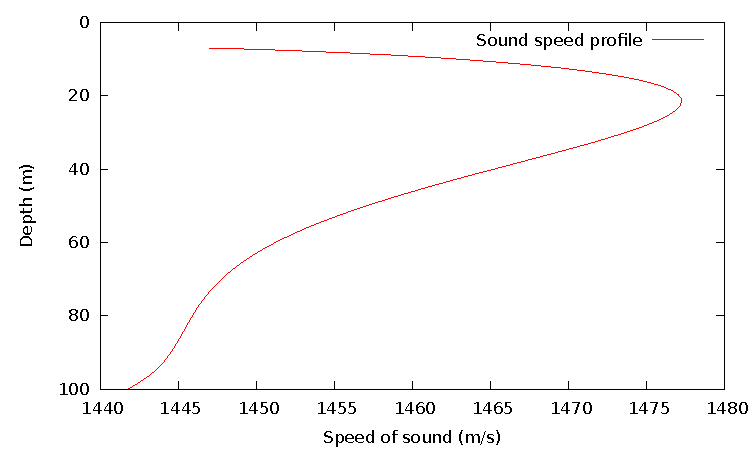
\includegraphics[width=3.5in]{../ssp.pdf}
  \caption{Sound speed profile}
  \label{fig:ssp}
\end{figure}

\subsubsection{Sources, Receivers, Ranges}
We base our study on the requirement that the network should be close
to the sea floor. We study the case in which there is only one
transmitter, in the middle and one receiver at a range of either 1km or
2km, at a depth between 87 and 92m. Therefore, we will have the
transmitter at 90m (5 meters above the bottom), the receivers at
depths between 87 and 92m in steps of 1m and at distances of 0.9km,
1.0km, 1.1km, 1.9km, 2.0km, 2.1km (to allow for variance).

\subsubsection{Bottom Description}
In this study, we use no specific data for the description of the
bottom composition. The bottom is treated as a rigid surface with an
inter-facial roughness of 0.2 m.

For the bathymetry, we use data from NOAA, the National Geophysical
Data Center. Since Bellhop can handle only 2D bathymetric data, we
transform the existing data to eight directions: N, NE, E, SE, S, SW,
W, NW. This data can be seen in table \ref{table:bty}.
\begin{table}
  \centering
  \begin{tabular}{|c|c|c|}
    \hline
    Direction & Range & Depth \\\hline
    E & 0 & 95 \\\hline
    E & 1.276 & 95 \\\hline
    E & 2.551 & 96 \\\hline
    SE & 0 & 95 \\\hline
    SE & 2.25 & 94\\\hline
    SE & 4.5 & 94 \\\hline
    S & 0 & 95 \\\hline
    S & 1.853 & 93\\\hline
    S & 3.706 & 93\\\hline
    SW & 0 & 95\\\hline
    SW & 2.25 &93 \\\hline
    SW & 4.5 &92\\\hline
    W & 0 & 95\\\hline
    W & 1.276 & 95 \\\hline
    W & 2.551 & 94 \\\hline
    NW & 0 & 95 \\\hline
    NW & 2.25 & 96 \\\hline
    NW & 4.5 & 94 \\\hline
    N & 0 & 95 \\\hline
    N & 1.853 & 97\\\hline
    N & 3.706 &95\\\hline
    NE & 0&95 \\\hline
    NE & 2.25& 97\\\hline
    NE & 4.5& 96\\\hline
  \end{tabular}
  \caption{\small{The Bathymetric values}}
  \label{table:bty}
\end{table}

\subsubsection{Run Type}
For our needs, we consider using the Amplitude-Delay file format,
given as option 'A'. This will provide us with the necessary arrival
paths for each source destination pair.

\subsubsection{Beam Width}
For this study, we use a beam width of $13^{\circ}$, between
$-10^{\circ}$ and $+3^{\circ}$. These values are based on previous
research in which it was found that there were no beams outside of
these angles. The number of beams is set to 0; this means that Bellhop
is free to choose an according value.

\subsubsection{Bounding Box}
As noted before, the bounding box should extend slightly besides the
ranges and the depths used in the model. In our case, the depths vary
between 92 and 97m and the maximum range is 2.1km. Therefore, the
bounding box was chosen to be at 100m vertically and 2.2km horizontally.

\subsection{Sample ENV file}
In this part, we will present a sample ENV file with the above
parameters. This file refers to a frequency of 1kHz.

\begin{verbatim}
'UWASN' !Title
1000 !Frequency
1 !NMEDIA
'CVFT' !SSP OPT
0 0 100 !Depth of bottom (m)
7 1447 /!SSP
10 1474.9 /
20 1497.7 /
30 1478.7 /
40 1460.1 /
50 1450.8 /
60 1447.1 /
70 1447.1 /
80 1444.9 /
90 1446.0 /
95 1443.8 /
100 1441.8 /
'R*' 0.02 /
1 !No. sources
90.0/ !Source depth
6 !No. receiver depths
87 88 89 90 91 92 / !Depths
6 !No. receiver ranges
0.9 1.0 1.1 1.9 2.0 2.1 / !Ranges
'A' !Run type
0 !No Beams
-10.0 3.0 /!Beam width
0 100 2.2 !Bounding box
\end{verbatim}

\subsection{Bellhop processing}
\label{subsec:bellhop}
The Bellhop processing requires input in terms of ENV files and BTY
files for the environment characteristics. Since we plan to use a
range between 0Hz and 60kHz, in steps of 250Hz, we need to run 240
files through Bellhop. Still, this is not enough, since we use 8
directions, each with its bathymetric description. Therefore we need
to run Bellhop through $1920 (240 \times 8)$ ENV files.

In order to take advantage of the technology advancement, the author
has designed a Makefile that can run in parallel Bellhop, as required
by the user. This is of great help, as with a quad-core processor with
simultaneous multithreading, one can run Bellhop 8 times in
parallel. Using such a processor, the author was able to achieve a
runtime of about 40 minutes for all the 1920 ENV files, in contrast
with the results provided in \cite{book} which yield a 25 hour runtime
on a dual-core processor.

The code base for this project resides at the URL \cite{github}, in
GitHub and is (or should be) thoroughly commented.

\subsection{Postprocessing}
\label{subsec:post}
Once Bellhop has been run over all the combinations fo ENV and BTY
files, the next step is to parse the resulting ARR files.

This is done via the \texttt{generate\_sig2noise.cpp} script which is
ran over an arrival file and generates multiple files of type
\texttt{val\_freq\_s\_r1\_r2\_bty.out}, where s is the source index (in
our case always 0), r1 is the depth index, r2 is the range index and
bty is the bathymetry index. These files contain values for the
transfer function, the dB value of the transfer function, the noise
value and the signal to noise ratio, for a certain $\langle$ frequency,
source, destination (depth and range) and bathymetry $\rangle$ tuple.

If we make a sweep through the entire frequency range, we will get
multiple files for a chosen sender receiver pair (multiple possible
bathymetries). The plot of the transfer function for one such file for
a case in which the source is 90m and the receiver is at 87m and a
range of 0.9km, on the North direction can be seen in figure
\ref{fig:hreal}. The value of the transfer function is obtained from
computing the absolute value of the $H(f)$.

\begin{figure}[ht]
  \centering
  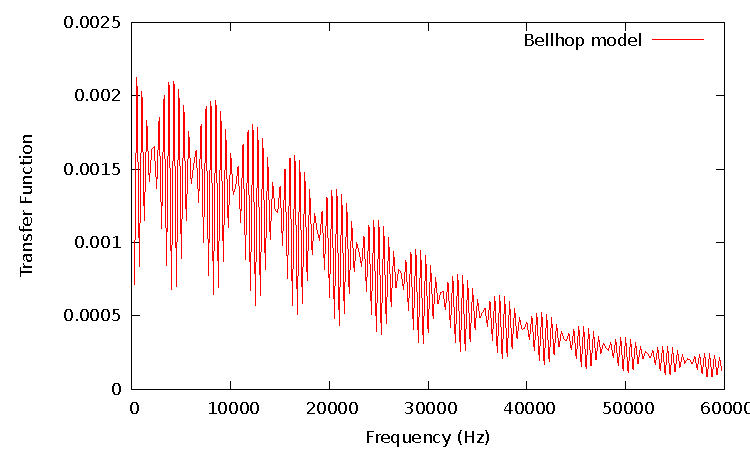
\includegraphics[width=3.5in]{../postprocessing/hreal00.pdf}
  \caption{\small{Transfer function value against Frequency for a
      single sender, receiver, bathymetry tuple}}
  \label{fig:hreal}
\end{figure}

Still, this plot is seldomly used, a more appropriate and relevant
plot being of the same data in a different scale, the dB scale. Such a
plot can be seen in figure \ref{fig:logh}.

\begin{figure}[ht]
  \centering
  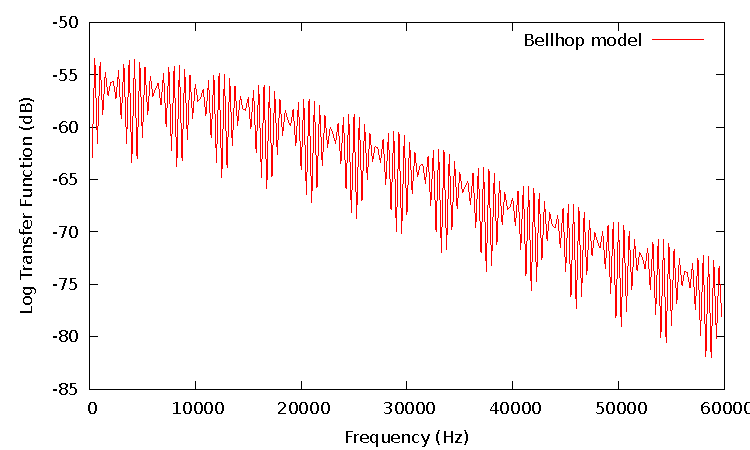
\includegraphics[width=3.5in]{../postprocessing/logh00.pdf}
  \caption{\small{Logarithmic transfer function value against
      Frequency}}
  \label{fig:logh}
\end{figure}

In both figure \ref{fig:hreal} and figure \ref{fig:logh}, we can see
that there is a tendency for a lower signal strength towards higher
frequencies. This is explained by the fact that, even though the
distance is stable, higher frequencies of the signal are attenuated
more, resulting in weaker signals.

The next value that is found in the file is the noise at a certain
frequency -- this value does not depend on anything else. The noise
function is computed using the formula in \cite{stojanovic}, using the
parameters $s = 0.5$ for shipping and $w = 0$ for wind, since we are
near the bottom of the sea and the wind and waves do not affect the
noise. A plot of the noise can be found in figure \ref{fig:noise}.

\begin{figure}[ht]
  \centering
  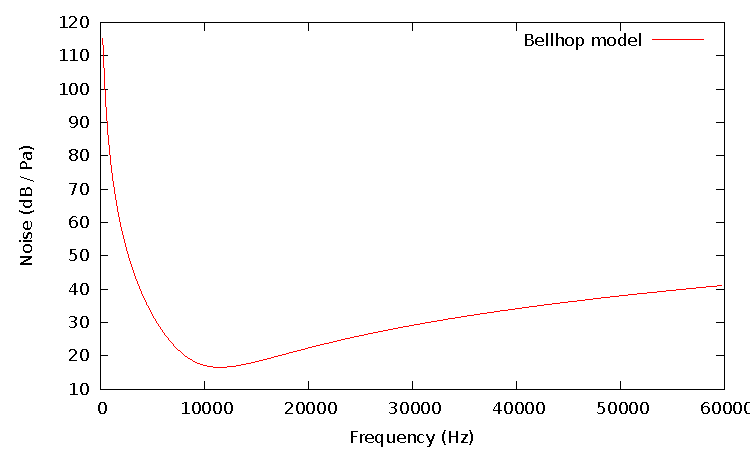
\includegraphics[width=3.5in]{../postprocessing/noise00.pdf}
  \caption{\small{Noise versus Frequency}}
  \label{fig:noise}
\end{figure}

The last value found in the files generated by this script is the
signal to noise ratio. A plot of this values can be seen in figure
\ref{fig:sig2noise}. As with the previous plots, towards higher
frequencies the signal strength is smaller and smaller, this being due
to the attenuation (which can be seen in the figure \ref{fig:logh}),
as well as due to the noise which increases at higher frequencies.

\begin{figure}[ht]
  \centering
  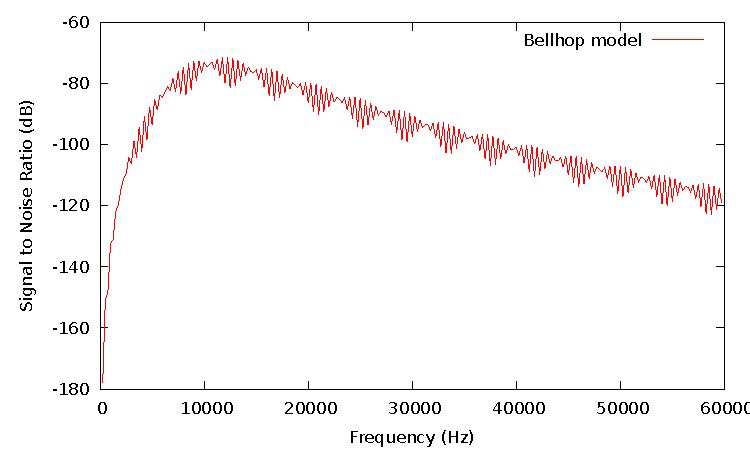
\includegraphics[width=3.5in]{../postprocessing/sig2noise00.pdf}
  \caption{\small{Signal to Noise ratio versus Frequency}}
  \label{fig:sig2noise}
\end{figure}

The final value that can be determined for a tuple of sender, receiver
depth, range and bathymetry is the capacity of the channel which will
tell us how much information can be transported. Given the bandwidth
(that is computed by one of the intermediary scripts), we can find the
center frequency (the frequency at which the signal to noise ratio is
highest) and the bandwidth (all frequencies within 3dB range). Given
this information, we can find out the capacity of the channel using
the formulas detailed in the previous section. We use a static source
power level of $180 dB re \mu Pa^2$. This results in a
plot like the one in figure \ref{fig:cap}. 

\begin{figure}[ht]
  \centering
  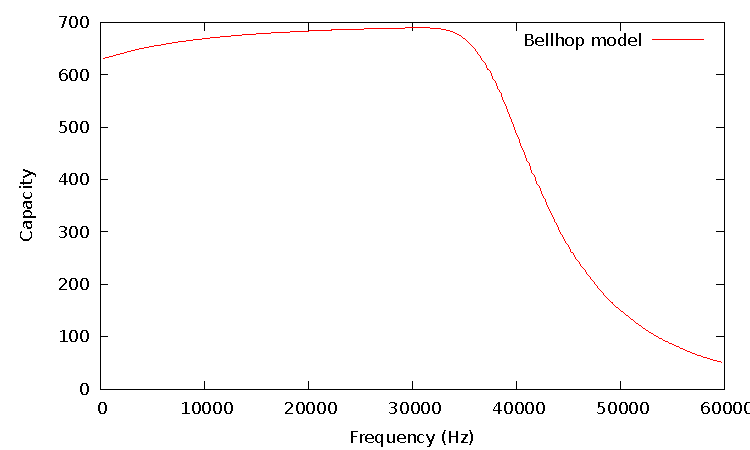
\includegraphics[width=3.5in]{../postprocessing/capacity00.pdf}
  \caption{\small{Capacity vs Frequency}}
  \label{fig:cap}
\end{figure}

We can see that near 30kHz the signal has the best capacity. This is
due to the fact that, according to our measurements, the bandwidth is
more than 50kHz on a regular basis, meaning that at 30 kHz, the entire
spectrum contributes to this value. Around, 40kHz the capacity
decreases abruptly. This is caused by the fact that the signal to
noise ratio also decreases towards higher values of the frequency,
therefore fewer, with less strength contributions are made towards the capacity.



\subsection{Depth based evaluation}
\label{subsec:depth}
%% varying the depth of the nodes -- how does it affect the bandwidth and
%%capacity
The results so far have only shown that towards higher frequencies,
there is greater attenuation and the signal strength is a lot
smaller. Still, frequency was the only parameter that we have changed
and this can extended. In this section, we propose changing the depth
of the receivers and see how the signal strength and capacity of the
channel are affected by this. The plot for the signal to noise ratio
can be found in figure \ref{fig:sig2noiseDepth}, while the plot for
capacity can be found in figure \ref{fig:capDepth}.

\begin{figure}[ht]
  \centering
  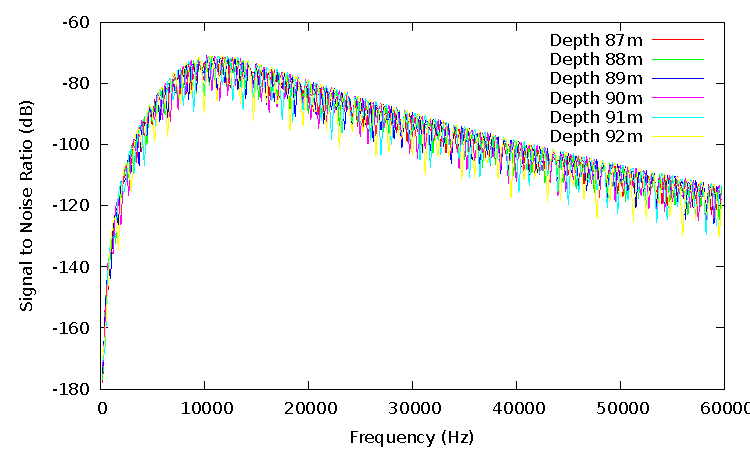
\includegraphics[width=3.5in]{../postprocessing/sig2noiseDepth.pdf}
  \caption{\small{Signal to Noise ratio against Frequency when the
      depth is modified}}
  \label{fig:sig2noiseDepth}
\end{figure}

\begin{figure}[ht]
  \centering
  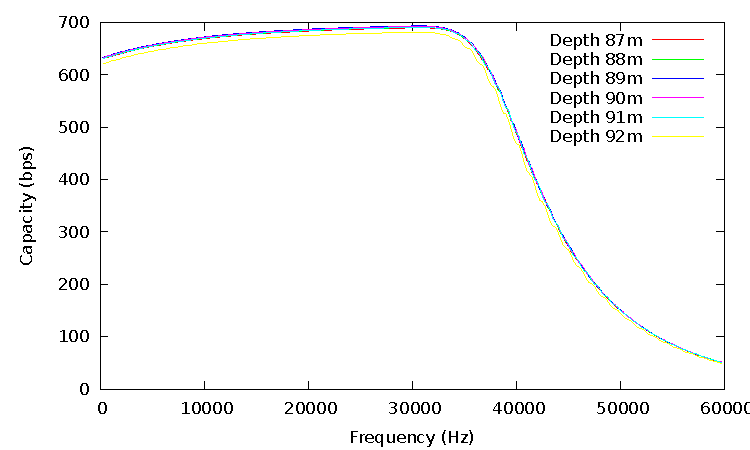
\includegraphics[width=3.5in]{../postprocessing/capacityDepth.pdf}
  \caption{\small{Capacity against Frequency when the depth is
    modified}}
\label{fig:capDepth}
\end{figure}

We can see from both plots that the change in depth in such small
scales has almost no effect on the channel, neither in signal
strength, nor in capacity. This might be because the distance between
the depth change is only 5m, while the distance between the source and
receiver is of 0.9km, rendering the change in depth insignificant.

\subsection{Range based evaluation}
\label{subsec:range}
%% varying the range -- how does it affect the bandwidth and capacity

The other parameter that we can change in our system is the range
between the source and the destination. We can vary that between the 6
possible values, between 0.9 and 2.1km and see how the signal strength
and capacity change. The plot of signal to noise ratio can be found in
figure \ref{fig:sig2noiseRange}, while the plot for capacity can be
found in figure \ref{fig:capRange}.

\begin{figure}[ht]
  \centering
  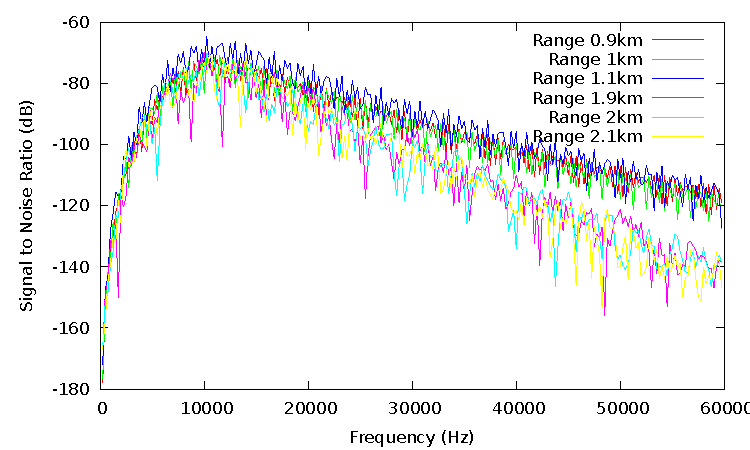
\includegraphics[width=3.5in]{../postprocessing/sig2noiseRange.pdf}
  \caption{\small{Signal Strength when varying the range}}
  \label{fig:sig2noiseRange}
\end{figure}

In figure \ref{fig:sig2noiseRange} we can see that at higher
frequencies there is a clustering for the two pairs of ranges -- near
1km and near 2km. This means that, as expected there is an inverse
relationship between the signal strength and the distance it
travels. This is explained by increased losses due to absorption,
spreading and reflective losses. In general, over higher distances,
higher frequencies are attenuated more than lower frequencies.

\begin{figure}[ht]
  \centering
  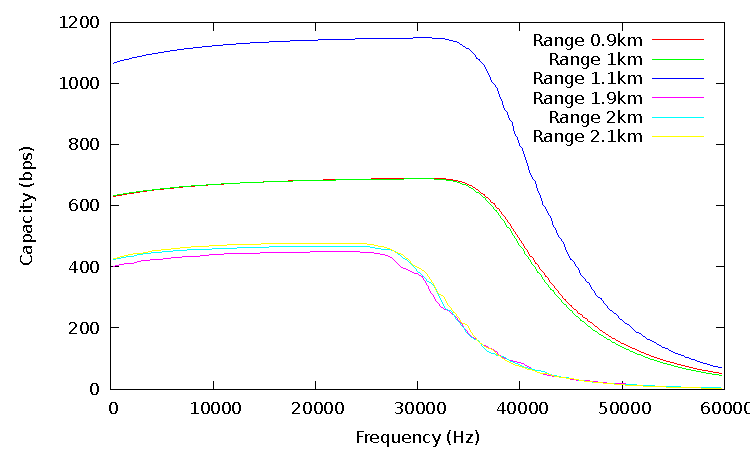
\includegraphics[width=3.5in]{../postprocessing/capacityRange.pdf}
  \caption{\small{Capacity when varying the range}}
  \label{fig:capRange}
\end{figure}

In figure \ref{fig:capRange}, we can see that the plot of capacity is
similar, just that the values near the 2km range are significantly
decreased. Besides the reasoning behind the signal to noise ratio
(which affects the capacity direclty), a narrowing of the bandwidth
can also be seen by an increase in range. Still, something very
interesting is happenning: the capacity at a range of 1.1km is almost
double the capacity at 0.9 and 1km. This can be explained by the
actual environment and that at that particular range, the multipath
effect is really strong and there are many rays that go between the
the source and destination.

\section{Conclusion and Future Work}

Prior knowledge of channel characteristics before deploying an
underwater sensor network is very important. Even more important is
that the environment is modelled as close to reality as possible,
using real life data for sound speed profile and bathymetry, so that
we can evaluate how the communication would be in real life and after
the network is deployed, what adjustments need to be made to the
modelling environment to better represent reality. 

In this paper, we have presented a comparison of how the depth and
range affect the transmission in an underwater environment, simulated
by the Bellhop modelling tool. We have seen that slight changes in depth of
the receivers do not affect the signal strength or the capacity of the
channel, since we are using only changes of 6m and ranges of 0.9 to
2.1km. Still, if we make a bigger impact on the depth of the nodes, we
might not have a near-seabed underwater network and the results will
vary.

As expected, by modifying the range between the two nodes, the signal
strength will have an inverse relationship with the range. This is due
to absorption and attenuation of the signal over large distances. This
effect is more noticeable towards high frequencies, which are more
attenuated than low frequencies.

This project can be enriched by several features, which are considered
further work:
\begin{itemize}
\item a measurement of how accurate is the Bellhop model with regards
  to reality would be very good
\item see how a change in bathymetry will affect the signal strength
  and capacity -- this has been studied in \cite{capacity}
\item one can use greater distances for the inter-node
  communication. 1 and 2km already show a change, but an increase to 5
  or 10 km might show an interesting change.
\item the Bellhop model is performing ray-tracing and therefore is
  really slow. A question is how accurate the data is and if other
  enhanced simulators, such as NS-2 \cite{ns2} which are a lot faster
  perform worse and how much worse.
\item the Bellhop model uses only the Thorp attenuation model which is
  builtin. Other attenuation models might yield better results.
\end{itemize}

\begin{thebibliography}{99}
\bibitem{capacity} \textit{A study of channel capacity for a seabed underwater
acoustic sensor network}, Peter King, Ramachandran Venkatesan, Cheng Li
\bibitem{model} \textit{An Improved Communications Model for Underwater Sensor
Networks}, Peter King, Ramachandran Venkatesan, Cheng Li
\bibitem{book} \textit{Channel Modelling for Underwater Acoustic Sensor
Networks}, Peter King, Ramachandran Venkatesan, Cheng Li -- Chapter 12 in
Underwater Acoustic Sensor Networks, Edited by Yang Xiao
\bibitem{nds} \textit{A Comparison of Channel Models for Simulating Underwater
Acoustic Communications}, Anuj Sehgal, Catalin David, J\"urgen Sch\"onw\"alder
\bibitem{stojanovic} \textit{On the Relationship Between Capacity and Distance
in an Underwater Acoustic Communication Channel}, Milica Stojanovic
\bibitem{bellhop} \textit{General description of the BELLHOP ray tracing program
(June 2008 release)}, Orlando Camargo Rodriguez
\bibitem{hayward} \textit{Underwater Acoustic Communication Channel Capacity: A
Simulation Study}, Thomas J. Hayward and T. C. Yang
\bibitem{ns2} \textit{Modeling the Underwater Acoustic Channel in ns2}, Albert
F. Harris III, Michele Zorzi 
\bibitem{oal} \url{http://oalib.hlsresearch.com/}
\bibitem{bio} \url{http://www.bio.gc.ca/}
\bibitem{noaa} \url{http://www.noaa.gov/}
\bibitem{ssp} \textit{Discussion of sea water sound‐speed
    determinations}, Kenneth Mackenzie in J. Acoust. Soc. Am. Volume
  70, Issue 3, pp. 801-806 (1981)
\bibitem{github} \url{https://github.com/cdavid/nds-channel-analysis}
\end{thebibliography}

\end{document}
